% -----------------------------------------------
% Template for ISMIR Papers
% 2018 version, based on previous ISMIR templates

% Requirements :
% * 6+n page length maximum
% * 4MB maximum file size
% * Copyright note must appear in the bottom left corner of first page
% * Clearer statement about citing own work in anonymized submission
% (see conference website for additional details)
% -----------------------------------------------

\documentclass{article}
\usepackage{ismir,amsmath,cite,url}
\usepackage{graphicx}
\usepackage{color}
\usepackage[ampersand]{easylist}

\setlength{\marginparwidth}{1.5cm}

\newcommand{\etc}{etc.}

% Title.
% ------
\title{Controlled Vocabularies for Music Metadata}

% Note: Please do NOT use \thanks or a \footnote in any of the author markup

% Single address
% To use with only one author or several with the same address
% ---------------
%\oneauthor
% {Names should be omitted for double-blind reviewing}
% {Affiliations should be omitted for double-blind reviewing}

% Two addresses
% --------------
%\twoauthors
%  {First author} {School \\ Department}
%  {Second author} {Company \\ Address}

%% To make customize author list in Creative Common license, uncomment and customize the next line
%  \def\authorname{First Author, Second Author}


% Three addresses
% --------------
% \threeauthors
%   {First Author} {Affiliation1 \\ {\tt author1@ismir.edu}}
%   {Second Author} {\bf Retain these fake authors in\\\bf submission to preserve the formatting}
%   {Third Author} {Affiliation3 \\ {\tt author3@ismir.edu}}

%% To make customize author list in Creative Common license, uncomment and customize the next line
%  \def\authorname{First Author, Second Author, Third Author}

% Four or more addresses
% OR alternative format for large number of co-authors
% ------------
\multauthor
{Pasquale Lisena$^1$ \hspace{.6cm}
Konstantin Todorov$^2$ \hspace{.6cm}
C\'ecile Cecconi$^3$ \hspace{.6cm}
Fran\c{c}oise Leresche$^4$ \hspace{.6cm}
} { \bfseries{
Isabelle Canno$^5$ \hspace{.1cm}
Fr\'ed\'eric Puyrenier$^4$ \hspace{.1cm}
Martine Voisin$^5$ \hspace{.1cm}
Thierry Le Meur$^3$ \hspace{.1cm}
Rapha\"el Troncy$^1$
}\\
$^1$ EURECOM, Sophia Antipolis, France \hspace{.7cm}
$^2$ LIRMM, University of Montpellier, CNRS, France\\
$^3$ Philharmonie de Paris, France \hspace{.7cm}
$^4$ Biblioth\`eque nationale de France \hspace{.7cm}
$^5$ Radio France\\
{\tt\small lisena@eurecom.fr, todorov@lirmm.fr, ccecconi@cite-musique.fr}
}
% \def\authorname{ }
\def\authorname{Lisena et al}

\sloppy % please retain sloppy command for improved formatting

\begin{document}

\maketitle

\begin{abstract}
We present a set of music-specific controlled vocabularies, formalized using Semantic Web languages, describing topics like musical genres, keys, or medium of performance. We have collected a number of existing vocabularies in various formats, converted them to SKOS and performed the interconnection of their equivalent terms. In addition, novel vocabularies, not available online before, have been designed by an editorial team. Next to multilingual labels and definitions, we provide hierarchical relations as well as links to external resources. We also show the application of those vocabularies for the production of vector embeddings, allowing for the calculation of distances between keys or between instruments.
\end{abstract}

\section{Introduction}\label{sec:introduction}
Describing music is an activity that involves an important number of terms coming from domain-specific glossaries. In addition to the cross-domain concept of genre, we can mention musical keys, instruments or catalogues of compositions. Libraries and musical institutions have different practices for describing this kind of information. In the best case, they make use of thesauri that are often available in different incompatible formats, and that can be either internally defined or standardised by larger communities such as the International Association of Musical Libraries (IAML). In other cases, this information is codified in free text fields, delegating to the editors the responsibility of following the living practice about syntax and lexical form.

The new attitude for sharing the knowledge beyond the institutional and national borders---embodied by international consortia like IAML or in projects like Europeana~\cite{europeana} and OpenGlam~\cite{estermann2016openglam}---brings its effect also on the music domain. Accordingly, Semantic Web technologies have gained a central role in music representation, that has reached the Linked Open Data world. A second consequence is the request for a change in the previously described current practices towards the adoption of publicly available controlled vocabularies.
The use of vocabularies opens up different possibilities, like the definition of labels in different languages or of alternate lemmata in the same language (i.e. the French terms ``ut majeur" and ``do majeur" which both refer to the key of \textit{C major}). Different kinds of relationships between terms can be defined and it is possible to define a hierarchy between them (for example, ``violin'' is a narrower concept with respect to ``string'') which can produce, as benefit, a more powerful advanced search for the final user. Previous research demonstrated how an RDF (for Resource Description Framework) structure helps reasoning engines to discover links between different levels in the hierarchy of instruments~\cite{kolozali2011knowledge}.

Publishing Semantic Web vocabularies is not new in the field of music. The Musical Instruments Museum Online (MIMO)\footnote{\url{http://www.mimo-db.eu/}} published the biggest taxonomy of musical instrument in RDF, as result of the contribution of institutions and universities all over the world. The librarian practice draws on the UNIMARC\footnote{They are commonly named after the UNIMARC standard for librarian records, in which they are widely used.} thesauri of musical forms (genres) and medium of performance standardised by IAML. Historically adopted by librarians worldwide, these thesauri have recently been published in the Web of Data, marking the growing interest in this technological environment. The French National Library (BnF) relies on an authority vocabulary in RDF for subject headings called RAMEAU,\footnote{R\'epertoire d'autorit\'e-mati\`ere encyclop\'edique et alphab\'etique unifi\'e: \url{http://rameau.bnf.fr/}} containing a list of labels for entities of encyclopedic interest which includes also music genres and instruments. A musical key vocabulary is published as side resource of the MusicOntology~\cite{raimond2007music}, consisting in a list of English labelled concepts, with some additional information---like the mode (\textit{major}/\textit{minor}), the tonic, \etc---, without any links describing semantic connections between them.

On the one hand, a large number of thesauri cover few well-defined categories (genres and medium of performance), making the reconciliation of data coming from different sources difficult, also because of the different formats of these thesauri. A reconciliation that would add a broader and deeper nomenclature has a benefit, increasing both the number of elements and alternate labels. On the other hand, a large set of concepts---handled so far through error-prone free-text---is asking for standardisation in specialised vocabularies.

This paper presents a set of controlled vocabularies for the description of the music information as Linked Open Data, extending and finalising related work in \cite{lisena2017modeling}. 
% These vocabularies have been collected and realised by the joint forces of an editorial team coming from libraries and musical institutions and academic laboratories in the field of Semantic Web.
% We not only demonstrate the completeness of those vocabularies, but we show how they can be used in various machine learning tasks such as empowering recommendation engines that would benefit from having a semantic vector representation of the metadata.
This research have the primary goal of the interconnection of music information datasets, building bridges between existing vocabularies and providing tools for the automatic matching. The final aim consists in the contribution to the achievement of a global music knowledge graph~\cite{doremusGraph} in the Web of Data, looking at all the applications that semantically structured data have in the music information retrieval and recommendation field~\cite{oramas2016recKG, oramas2017cold, Weigl2017AFF, MusicLynx}.
In \secref{sec:vocabularies}, we present the complete set of vocabularies, giving detailed information about their content. The process of realisation, collection and interlinking is described in \secref{sec:realisation}, while we present applications, such as embeddings and literal dereferencing in \secref{sec:usage}. Finally, we conclude and outline some and future work in \secref{sec:conclusion}.


\section{Music Vocabularies}\label{sec:vocabularies}
A controlled vocabulary is a thematic thesaurus of entities. In the Semantic Web, each term is identified with a URI. The \textit{Simple Knowledge Organization System (SKOS)}~\cite{miles2007skos} have been chosen as format because of its capability of defining preferred and alternate labels in each language, relationships between terms, comments and notes for describing the entity and help the annotation activity.
In the case of the vocabulary of \textit{Catalogues of works}, the used ontology is the RDF version of \textit{Metadata Object Description Schema (MODS)}~\cite{mods-specification}, that suits the need of defining identifiers, publication date, subject, \etc

Each vocabulary fulfils a set of requirements, including multilingualism, open and public access, presence of definitions. It must also be suitable for different contexts of use and conceptual models of musical information, which is guaranteed by the presence in the editorial team of experts from different types of cultural institutions (libraries, radio broadcasting networks, concert halls).

The vocabularies are all available in a triple store server, which provides a SPARQL endpoint\footnote{\url{http://data.doremus.org/sparql}} for requesting the data in different formats like RDF, JSON, csv, etc. Alternatively, the vocabularies can be explored by a web browser starting from
\url{http://data.doremus.org/vocabularies/}.
The server enables the HTTP dereferencing of URIs: this means that a web browser pointing to the URI of a specific concept (e.g.
\url{http://data.doremus.org/vocabulary/derivation/medley}) will land on a page containing its human-readable description, showing all its properties. The triple store includes also music data that use these vocabularies, so that the definition and the usage of a concept in musical works can be appreciated as part of the same knowledge base. Finally, an RDF version in Turtle format is available on GitHub.\footnote{
\url{https://github.com/DOREMUS-ANR/knowledge-base/tree/master/vocabularies}
}

Each vocabulary is licensed for free distribution, following a Creative Commons Attribution 4.0 license,\footnote{\url{https://creativecommons.org/licenses/by/4.0/}} and it is open to the community for any kind of contribution.  

We collected, implemented and published 18 controlled vocabularies belonging to 7 different families, containing more than 9500 distinct concepts and involving 26 different languages or dialects. In the following paragraphs, we describe the content of those vocabularies, subdivided in two groups.

\subsection{Collection of interlinked vocabularies}\label{sec:collection}
This group includes vocabularies that were already available in the Web of Data, in the community or internally to a specific institution. When two or more vocabularies share the same high-level topic---e.g. the musical genre---we call that group \textit{family}. In order to interconnect the different knowledge sources, an alignment process is needed for discovering when terms coming from vocabularies belonging to the same family refers to the same concept. This process will be detailed in \secref{sec:interlinking}.

\vspace{-0.3cm}
\paragraph*{Musical genres.} This family includes vocabularies about the genre of a musical work. By genre, we mean the main categories by which we describe the works, like rock, lirica, funk, opera, gospel, polka, jazz, including genres of world music. The term genre is very broad and also includes musical ``forms" that gained in the centuries their own genre definition like symphony, concerto, sonata.

We collected, republished as SKOS and interlinked the following vocabularies:
\begin{easylist}[itemize]
\ListProperties(Space*=0pt, Margin=0ex)
& \textbf{IAML}, 607 concepts, multilingual. This list, largely adopted in librarian environments, was available as a set of labels and codes, in some cases with definitions or editorial notes. We converted this big vocabulary to SKOS from different sources (librarian tabular data, online HTML version). Afterwards, a SKOS version\footnote{\url{http://iflastandards.info/ns/unimarc/terms/fom/}} has been published by IFLA (International Federation of Library Associations), which is however less rich than ours in terms of alternate labels. We provide \texttt{owl:sameAs} links from our vocabulary to the IFLA version.
& \textbf{RAMEAU}, 654 concepts, French, hierarchised. It is published as Linked Data by the French National Library (BnF). We extracted from this large nomenclature the part related to musical genres.
& \textbf{Diabolo}, 629 concepts, French, hierarchised. It is the set of labels used in the disc catalogue of Radio France (RF). It also includes some \texttt{skos:related} links, e.g. between \textit{spiritual} and \textit{gospel}.
& \textbf{Itema3}, 40 concepts, French. It is used in the technical documentation of the concert archive of RF.
& \textbf{Itema3-MusDoc}, 172 concepts, French. It is used in the musical documentation of the concert archive of RF.
& \textbf{Redomi}, 297 concepts, French, hierarchised. It is used in the musical work documentation of RF.
\end{easylist}

\vspace{-0.3cm}
\paragraph*{Medium of performance.}
Any instrument able to produce sounds can be considered as a medium of performance or MoP. In this family of vocabularies, we can find musical instruments coming from different cultures (western, oriental, African, Indian, \etc), the voices in different ranges (soprano, alto, \etc), aside from group of instruments (orchestras, ensembles) and voices (choirs).

We collected, republished as SKOS and interlinked the following vocabularies:
\begin{easylist}[itemize]
\ListProperties(Space*=0pt, Margin=0ex)
& \textbf{MIMO}, 2480 concepts, multilingual, hierarchised. The \textit{Musical Instrument Museum Online} comes from the joint international effort of different music institutions and museum. Despite being the most complete vocabulary of instruments, it does not include voices. MIMO is publicly available as Linked Data.\footnote{\url{http://www.mimo-international.com/}}
& \textbf{IAML}, 419 concepts, multilingual, hierarchised. Despite its smaller granularity, this vocabulary has a good coverage for voices and groups. Like for the homonym genre vocabulary, also in this case an official version from IFLA is online,\footnote{\url{http://iflastandards.info/ns/unimarc/terms/mop/}} less rich both with respect to the languages covered and to the number of concepts (392).
& \textbf{RAMEAU}, 876 concepts, French, hierarchised. As in the genre case, we selected the part related to MoP.
& \textbf{Diabolo}, 2117 concepts, French, hierarchised. It is the set of labels used in the disc catalogue of RF. For ethnic or traditional instrument, it includes also the reference to the relative geographic area.  
& \textbf{Itema3}, 314 concepts, French. It is used in the documentation of the concert archive of RF.
& \textbf{Redomi}, 179 concepts, French, hierarchised. It is used in the musical work documentation of RF.
\end{easylist}

\subsection{New vocabularies}\label{sec:newvoc}
This section presents vocabularies for which we did not rely on any previous material, because it was not existing or not suitable for our goals. We designed these vocabularies on the basis of real data coming from institutions, enriched by an editorial process that involved also librarians. Since the work has been conducted in French, the definitions of the terms are so far available only in this language. However, every label has been translated at least in English and Italian in order to facilitate their reuse.

\vspace{-\baselineskip}
\paragraph*{Musical keys.} 30 concepts, English, French, Spanish, Italian.
This vocabulary contains the set of keys used in western music, labelled with the tone followed from the type of scale (e.g. \textit{C major}). The concept are linked among them by specific properties for keys relationships, like \textit{relative}, \textit{parallel} and \textit{closely related} keys. It contains also \texttt{sameAs} links with the key vocabulary of MusicOntology.

\vspace{-\baselineskip}
\paragraph*{Musical modes.} 22 concepts, English, French, Italian, Latin, hierarchised.
The word \textit{mode} generally refers to a type of scale, coupled with a set of characteristic melodic behaviours. They are mostly used for describing ancient or medieval music.

\vspace{-\baselineskip}
\paragraph*{Catalogues of works.} 152 MODS resources.
A \textit{thematic catalogue} or \textit{catalogue of works} is a recognised editorial list of all known works of a composer. In practice, a classical composition can be univocally identified by the catalogue code and number. For example, \textit{Eine kleine Nachtmusik} is identified with \textit{K 525}, where \textit{K} is the K\"{o}chel catalogue of Mozart's work. Each resource contains the information about the catalogue editor and publisher, the language of drafting, the date of publication. The subject artist of each catalogue is disambiguated through the DOREMUS dataset~\cite{lisena2017modeling, doremusGraph}.

\vspace{-\baselineskip}
\paragraph*{Types of derivations.} 16 concepts, English, French, Italian, Spanish, German, hierarchised.
A work can be derived from another by transforming its material into another through orchestration, harmonisation, etc. All these types (with definitions) are collected in this vocabulary.

\vspace{-\baselineskip}
\paragraph*{Functions.} 106 concepts, English, French and Italian, hierarchised.
A music event---a performance, a composition, a recording, etc.---involves a number of different roles or \textit{functions} like author, performer, conductor, sound engineer, \etc Additional details can also be provided to account for the different kinds of author, like composer, lyricist or arranger. These functions are identified in this vocabulary, together with their definitions.

\section{Modeling process}\label{sec:realisation}
We detail the modeling process, which is based on an interaction between music metadata experts and automatic data conversion and fusion tools.

\subsection{Editorial work}
An editorial committee grouping 7 members coming from different backgrounds (library, radio, concert hall) played an important role in the vocabulary modeling. First, existing vocabularies have been inventoried and assessed as candidates for being interlinked on the basis of their completeness and adoption. Next, the committee made choices about which new vocabularies to create and what should be their scope. These choices reflect the aim of producing powerful tools to describe recordings, publications and their contexts of creation, instead of producing exhaustive vocabularies about every aspects of the music. The committee relies on the members experience in music data management practices. The experts had to confront their point of views---necessarily different because depending on the missions of their institutions---until the list of terms, their contexts of use and their definitions were coherent.

First of all, the group had to be consistent with respect to the data available in those institutions. For example, we chose not to publish a rhythmic patterns vocabulary since the data which is available was not created in a musical analysis perspective. Then, the work had to be based upon the team's area of competence. This is one of the reasons why we decided to limit the scope of the musical modes vocabulary to old and European ones only. Listing and describing scales coming from other continents would require an additional work that would largely involve musicologists. 

We chose first to create the new vocabularies described in \secref{sec:newvoc}. The catalogues of works vocabulary is a special one since it contains only a list of bibliographic references and does not have the structure of a thesaurus. It was established from the titles used by the BnF. The musical keys and musical modes vocabularies were the easiest to model since they contain a small number of well-defined concepts with clear translations. The other ones were more complex to model. A first set of entities was generated on the basis of the initial datasets. Then, the experts had to confront their point of views until the list of terms, their contexts of use and their definitions were coherent. The functions vocabulary was especially complex to define since it had to reconcile very different ways of describing performing art activities: What is the relevant description for ``sound engineer"? How to describe the act of improvising? \etc 

\subsection{Conversion to Semantic Web formats}
Two different steps take part in the generation of the vocabularies as RDF graphs.

The first one is a preliminary conversion from spreadsheets or XML files to RDF, using the OpenRefine~\cite{ham2013openrefine} tool or with specific scripts. The collections of concepts already in the Web of Data (like RAMEAU) have been instead extracted through specific SPARQL queries on an endpoint.

In the second step, additional vocabulary-specific actions are performed. In some cases, hierarchy is inferred on the basis of specific properties and rules (e.g. in the IAML MoP vocabulary, the hierarchy is taken from the letters included in the last part of the URI).
All the language tags are normalised in order to follow the ISO 639 standard. Moreover, the indication of the use of Latin script is made explicit for transliterated labels in languages that use different alphabets.
In this phase, some interlinking to external datasets is performed, using SPARQL queries (DOREMUS dataset, MusicOntology keys vocabulary) or REST APIs like GeoNames~\cite{wick2012geonames}.

\subsection{Vocabulary Alignments}\label{sec:interlinking}
The sets of vocabularies of musical genres and those of medium of performance, described in \secref{sec:collection}, group together a number of well-established or internally used within a given institution reference lists. There is an important overlap between the sets of entities (genres or musical instruments) described across these vocabularies in each of the two categories. For example, the music genre ``folk song" is described both in the IAML vocabulary (labelled by the French ``chanson populaire" and the English ``folk song") and in the Radio France-hosted Diabolo vocabulary (labelled by ``folksong"). The task of vocabulary alignment consists in automatically establishing links of identity between the elements of two vocabularies from the same category. This would allow to discover automatically the equivalence between the two folk-song terms across IAML and Diabolo. Since our vocabularies are described in SKOS, the procedure comes down to discovering and declaring {\tt skos:exactMatch} relations across the terms of two given vocabularies. In our example, this would result in bounding the IAML and Diabolo identifiers\footnote{Respectively,
\url{http://data.doremus.org/vocabulary/iaml/genre/fso} 
and 
\url{http://data.doremus.org/vocabulary/diabolo/genre/folksong}
} of the folk-song genre in a  {\tt skos:exactMatch} relation.

We have proceeded to establish pairwise alignments between the concepts of the vocabularies in each of these two categories (genres and MoP). We have chosen IAML as a target vocabulary for the alignments of the genres-vocabularies, meaning that all remaining genre-vocabularies will be aligned to IAML. This decision is motivated by the fact that this vocabulary is large in size and also largely adopted in the librarian world. In the same line of thought, we have selected MIMO from the MoP family as a target for the alignments. This results in the performance of five pair-wise alignments for each category (all to IAML in the genre category and all to MIMO in the MoP category).

\begin{figure}[h]
	\centering
		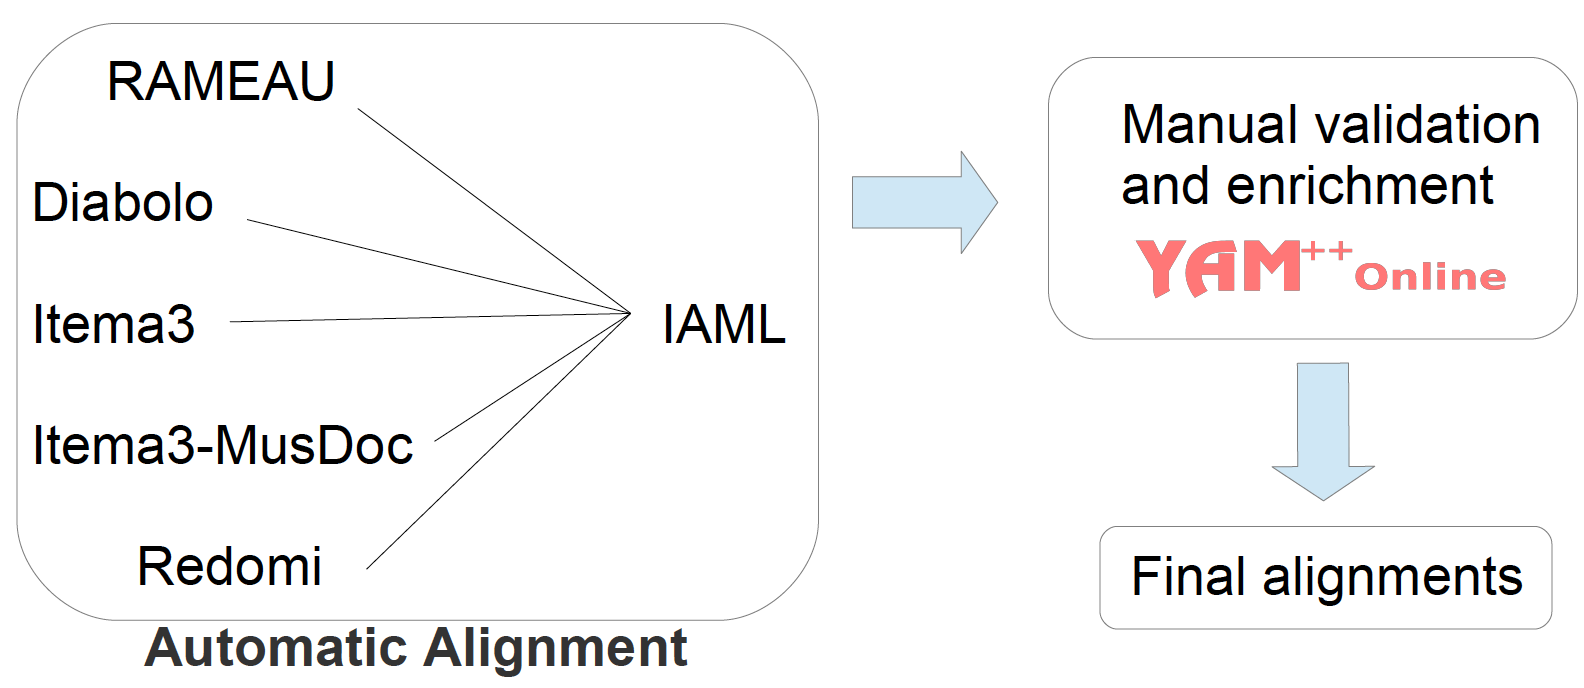
\includegraphics[width=7cm]{figs/pipeline.png}
	\caption{The overall alignment and expert-validation framework. An example with the genres family.}
	\label{fig:alignPipeline}
\end{figure}

The overall alignment process consists of {\it automatic alignment} and {\it manual validation and enrichment} (see \figref{fig:alignPipeline}). For the automatic alignment, we have taken a simplistic string-based approach that relies on a comparison between the labels of SKOS concepts by looking both at preferred and alternative labels, returning in output a confidence score. Note that in many cases, we have language tags associated to the terms. However, there is no consensus among the different vocabulary providers on the language of origin of the terms of interest -- in many cases a  musical instrument or a genre will be labelled as ``French" in one vocabulary and ``Italian" in another, although the label originates in, say, Italian in both cases, simply because the Italian word is commonly employed in French. For that reason, we have ignored the language tags when comparing the labels. This process aims to generate a large pool of mapping candidates, ensuring high recall at this step. The alignments are stored in the standard EDOAL format,\footnote{\url{http://alignapi.gforge.inria.fr/edoal.html}} which allows to keep the confidence score of each aligned pair of terms.

\begin{figure*}
	\centering
		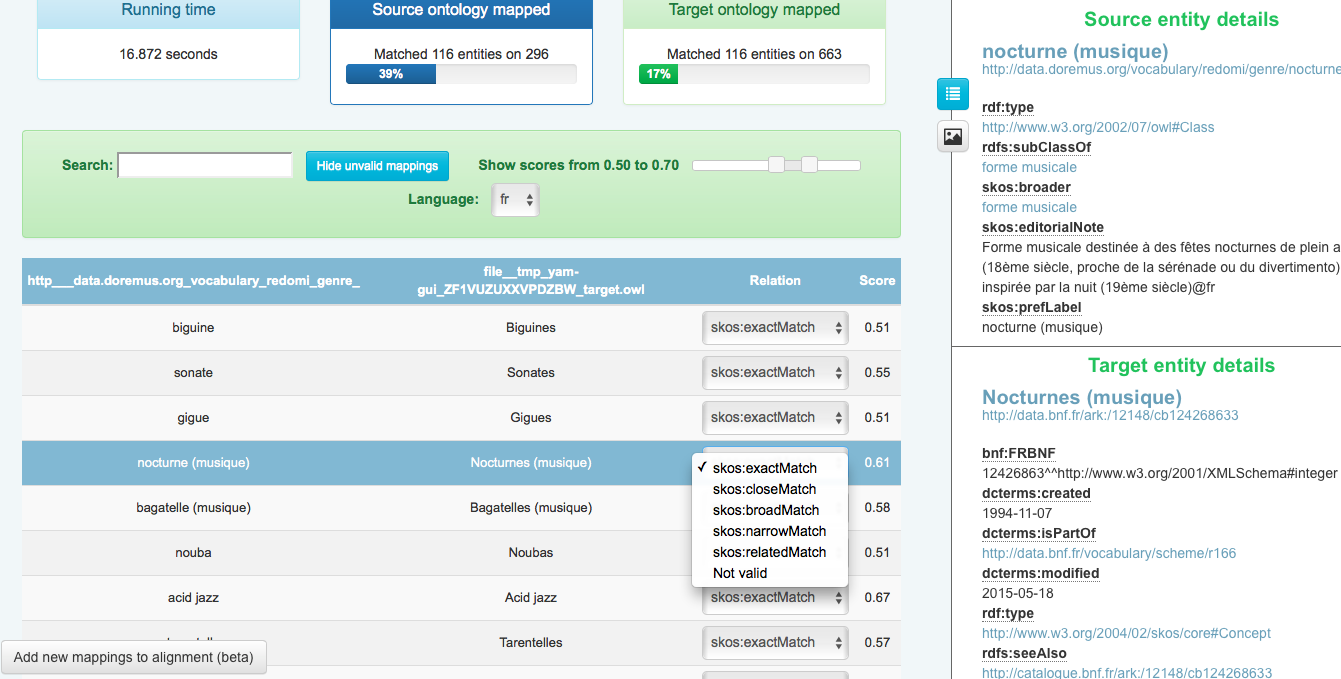
\includegraphics[height=5cm]{figs/screen2.png}
	\caption{The mapping validator interface.}
	\label{fig:screen2}
\end{figure*}

In order to guarantee high quality of the produced alignments and to improve precision, the automatically generated mappings are subjected to validation by the librarian experts. In order to facilitate this laborious task, we have developed a web application that allows to assist this process. The application has been conceived as a module of YAM++ {\it online} \cite{bellahsene2017yam++}---a multi-task web platform for ontology and thesaurus matching and validation,\footnote{
\url{http://yamplusplus.lirmm.fr}
} although the {\bf Validator} interface can be seen as a standalone tool. It takes as input a valid EDOAL alignment file, together with its two OWL ontologies or SKOS vocabularies (via an URL or a file path). A list of mappings (pairs of labels of aligned concepts) appears on the main page, together with information about the portions of the vocabularies covered by the alignment (\figref{fig:screen2}, above). A context description of each of the two concepts in each line is displayed (\figref{fig:screen2}, right), containing all alternate labels, as well as the labels (or URIs) of parents and children. The user can take benefit of the confidence score of the previously computed alignments (shown at the right end of each line) for filtering the pairs of concepts by the help of a horizontal cursor. For each concept pair, the expert is given the possibility to modify and select a relation type from a list of SKOS relations, or simply discard the mapping. Experts spotted out and corrected a number of invalid alignments (507 over 1022 for genres and 2039 over 3981 for MoP). In particular for small differences in the label (i.e. plural forms) the role of the human validation is crucial for ensuring quality in the vocabularies.

The expert is given the possibility to manually enrich the proposed alignment by the help of the alignment enrichment environment, accessible via the ``Add new mappings" button (\figref{fig:screen2}, bottom left). A new page opens containing the full label lists of the two vocabularies. A key-word search on both lists, including preferred and alternate labels, allows to browse and select manually a pair of concepts and define their relation. The newly defined mappings are added to the initial alignment. Finally, all modifications are added to the alignment file, which can be either saved in the default EDOAL format, or exported in the form of RDF/XML triples.

\section{Usage of vocabularies}\label{sec:usage}
The availability of controlled vocabularies opens up new possibilities that involve the data conversion and usage. In this section, we present recent work that aims to be complementary to the vocabulary publishing, providing further tools and resources to support their effectiveness.

\subsection{String2Vocabulary}
A common task in what is called \textit{knowledge graph population} (which is the generation of semantic triples starting from differently structured data sources) is the passage from plain text nodes or \textit{literals} to a more representative object node or \textit{entity}. Often, the target of this task consists in a set of vocabularies.

A \textit{string2uri} algorithm -- developed in the context of the Datalift platform~\cite{scharffe2012enabling} -- performs an automatic mapping of string literals to URIs coming from controlled vocabularies in SKOS. The software reads a RDF graph and searches for exact matches between literal nodes and vocabulary terms.

Some experiences in knowledge base population of classical music data, have shown up some critical points. Often the title of a classical work includes or, even more, consists in the name of an instrument or a key or a genre (e.g. Ravel's \textit{Bolero}), that should be excluded from the replacement process and be kept as textual literals. Moreover, the complexity itself of this data -- involving an important number of properties -- in addition to the commonly used file formats (i.e. MARC), has led in the years to a cataloguing practise particularly prone to editorial mistakes. This is the case of musical keys declared as genre, or fields for the opus number that contain actually a catalog number and vice-versa~\cite{lisena2017modeling}.

For these reasons, we adapted the Datalift strategy in a new \textit{String2Vocabulary} open-source library.\footnote{
\url{https://github.com/DOREMUS-ANR/string2vocabulary}
} The software uses the file name of vocabularies for grouping them in families: \textit{mop-mimo.ttl} and \textit{mop-iaml.ttl} are part of the family \textit{mop}, while \textit{key.ttl} is the sole member of the family \textit{key}.
This library accepts a configuration file that assigns a family to a RDF property. For each input graph, it searches for the properties one after the other, retrieving their values. Each value is then compared to all the terms of the vocabulary, until it finds one equal to the value. All variants for a concept label -- namely \texttt{skos:prefLabel} and \texttt{skos:altLabel} -- are considered in order to deal with potential differences in naming terms, and both graph values and terms receive a normalisation that has the effect of removing the punctuation, lower-casing the text and decoding it to ASCII. Then, a substitution of that node with the found concept URI is performed.

\textit{String2Vocabulary} works both with literal values and with entities labelled through \texttt{rdfs:label}. In the latter case, the label to be matched against the vocabulary and the whole node -- with all its properties -- is replaced.
For maximising the possibilities of selecting, if it exists, the right concept, two searches are performed in sequence. The first requires that both the given text and language match with the concept ones. If this search fails, a second one requires a match excluding the language information.

As additional feature, the configuration file allows to request the lemmatisation for certain vocabularies. Taking the MoP vocabulary as representative example, three sequential matches are tried: singularising the first word of the label (for matching cases such as \textit{``cornets \`a pistons"@fr}), singualising the whole label (\textit{``sassofoni contralti"@it}) and leaving the label as is for matching instruments that are always plural (\textit{``cymbals"@en}). 

\subsection{Music Embeddings}
What are the closest keys to \textit{C major}? Is it possible to decide which instrument between the \textit{cello} and the \textit{oboe} is more similar to the \textit{clarinet}? The answer to those questions would provide application in different fields, from musicology studies to the development of specialised recommendation systems. The graph structure of RDF allows to define some kind of distance between two entities, by considering the number of nodes that separate them. Hierarchies and other kind of links between vocabulary terms can be considered for computing this distance.

\textit{Node2vec}~\cite{node2vec-kdd2016} is a state-of-the-art algorithm for computing entity embeddings. The algorithm computes random walks in the graph following the links (\text{edges}) between nodes, computing the neighbourhood for each of them. Each edge can have a different \textit{weight}, which affects the probability that it participates to the walk. Through this method, the graph is mapped to a vector space, in which nodes becomes points represented by numeric vectors.

A set of music embeddings for the concepts defined in controlled vocabularies are being produced and published.\footnote{
\url{https://github.com/DOREMUS-ANR/music-embeddings}} 
Two different graphs are considered:
\begin{easylist}[itemize]
\ListProperties(Space*=0pt, Margin=0ex)
& the graph of vocabularies, which defines structural and semantic connections between entities, such as hierarchies, \texttt{sameAs} links, properties in common, specific music properties (i.e. relationships between keys);
& the graph of usage, which includes all the usages of the vocabularies in the DOREMUS dataset. We considered musical works for the genre and the key, castings and performances for MoPs, composition and performance events for functions.
\end{easylist}

On these two graphs, we computed the embeddings using \textit{node2vec}. We arbitrarily set to the graph of vocabularies a weight 6 times bigger than the graph of usage in order to counterbalance the richly larger number of triples\footnote{More than 16 millions triples against around 100.000 ones for the vocabulary graph.} and avoid to nullify the contribution of each one. After a post-processing step that removes all the literals and the extra nodes involved, a L2 normalisation is then applied in order to have values in \{-1;+1\}.

In order to appreciate the effectiveness of this strategy, we used t-SNE~\cite{maaten2008visualizing} for visualising the embeddings on a 2D image. As an example, \figref{fig:mop-space}\footnote{A higher-resolution image is available at 
\url{https://github.com/DOREMUS-ANR/music-embeddings/tree/master/img}} shows the vector space of \textit{medium of performance}. By observing the groups of closer entities, we can clearly identifies clusters of instruments. It is interesting to observe that even if the hierarchy of the instrument families is preserved, the usage graph strongly influenced the result, by reflecting the differences of instruments in genres and periods. This is the case of the orchestra instruments group, which puts the \textit{violin} closer to his orchestra colleague \textit{clarinet} than to its 15$^{th}$-century relative \textit{tromba d'amore}.

\begin{figure}
	\centering
		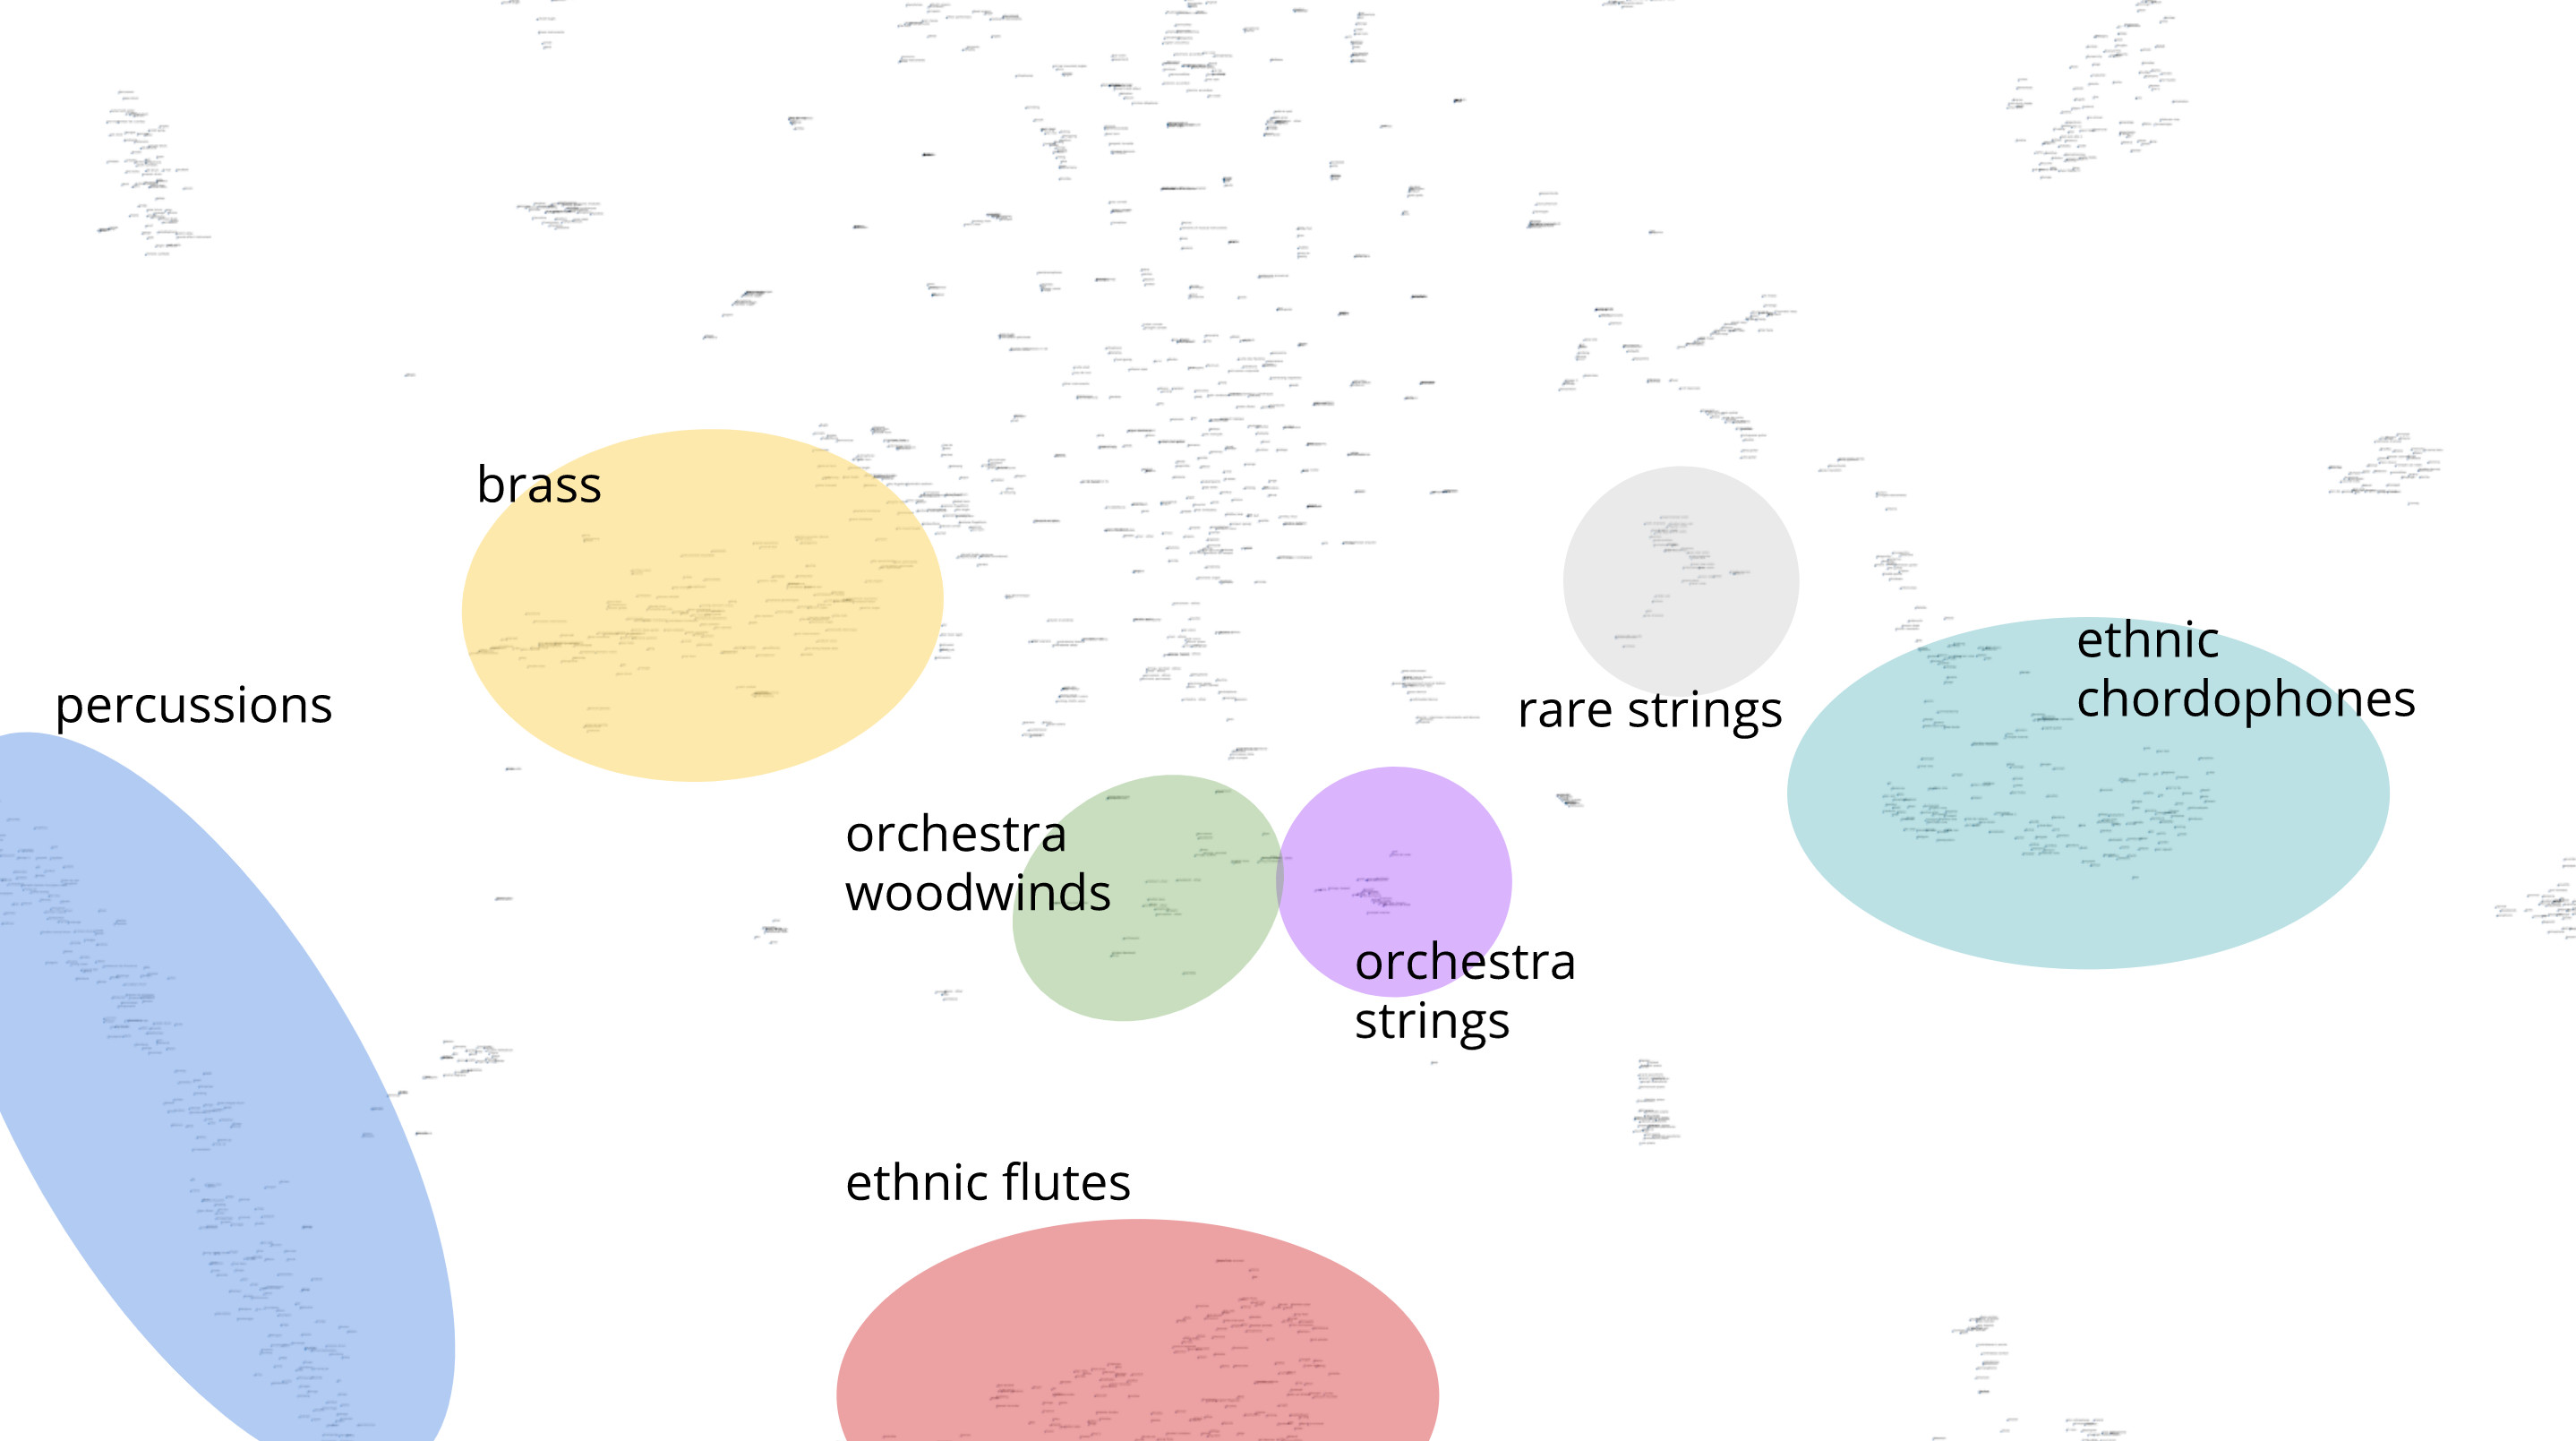
\includegraphics[width=\columnwidth]{figs/map-mop.jpg}
	\caption{A 2D representation of the vector space of \textit{medium of performance}, with some recognisable clusters.}
	\label{fig:mop-space}
\end{figure}

Further research is being conducted about the combination of this embedding in more complex ones (artists and works embeddings) in order to compute the similarity between musical entities~\cite{lisena2017artistsimilarity}.

\section{Conclusion}\label{sec:conclusion}
We have presented a set of multilingual vocabularies for the description of music-specific concepts using the Semantic Web framework. Two main contributions consist in the interconnection of already in-use vocabularies of genres and medium of performance and the realisation of previously-unreleased ones. We described our working strategies as an interaction between editors and an automatic system. A dereferencing library and a set of embeddings are presented as side works, allowing to identify application benefits coming from these vocabularies. 

Those vocabularies are intended to become references in the field and we strongly encourage their reuse and adoption by the community at large in all their forms. Several additional vocabularies are currently under development, covering concepts like vocal techniques, types of work, type of recording support or partitioning of musical works. Once completed, these vocabularies will be published by following the procedures described in this paper.

\paragraph*{ACKNOWLEDGMENTS} This work has been partially supported by the French National Research Agency (ANR) within the DOREMUS Project, under grant number ANR-14-CE24-0020.

% For bibtex users:
\bibliography{bibliography}

\end{document}
